% Author: Alexander Svozil
% Matr.-nr.: 1026213
% TU Wien
\documentclass [12pt]{article}
\usepackage [utf8]{inputenc}
\usepackage {graphicx}
\usepackage{algorithm}
\usepackage{algpseudocode}
\usepackage{amssymb}
\usepackage{tikz}
\usepackage{float}
\usepackage{pgfplots}
\usepackage{setspace}

\usetikzlibrary{shapes.multipart}

\bibliographystyle{ieeetr} 
\renewcommand{\algorithmicrequire}{\textbf{Input:}}
\newtheorem{mydef}{Definition}
\begin{document}
\vspace{20pt}
\begin{center}
  \fontsize{45pt}{25pt}\selectfont Bachelor Thesis 
\end{center}
\vspace{50pt}
\begin{center}
  \fontsize{55pt}{30pt}\selectfont\textbf{The Server Location Problem with Restricted Loads on Servers and Links} 
\end{center}
\vspace{50pt}

\begin{center}
\large Alexander Svozil (1026213)\\April 10, 2014
\end{center}
\vspace{20pt}
\begin{center}
\large Institute of Computer Graphics and Algorithms (E186) at the Vienna University of Technology 
\end{center}
\vspace{20pt}
\begin{center}
\large Field of work: Algorithms and Datastructures \\ Supervisor: Univ.-Prof. Dipl.-Ing. Dr.techn. Günther Raidl \\
\end{center}
%\maketitle
\thispagestyle{empty}
\newpage


\section*{Abstract}
The server location problem with restricted loads on servers and links (SLRL) is an NP-complete
problem, introduced by Miwa et al. The problem 
is motivated by the fact that a massive volume of data distributed by content delivery networks (CDNs) 
requires well located mirror servers in order to render a satisfactory performance in terms of quality of service.
Two constraints important for the choice of mirror servers is (i) the number of maximum nodes
accessing a mirror server and (ii) the maximum number of nodes accessing a mirror server 
through a specific link. The constraint mentioned first limits the network load on
the (mirror-)servers. The second constraint restricts the load on the links.
The problem will be formally defined, some background information will be given and SLRL will be shown to be NP-complete.
Then heuristic algorithms based on tabu search and simulated annealing will be introduced and their performances will be evaluated in comparison with the algorithm proposed 
by Miwa et. al. 

\thispagestyle{empty}

\newpage
\tableofcontents
\newpage


\section{Introduction}
\subsection {CDNs}
The CDN also content delivery network is a collaborative collection of network elements.
To perform transparent and effective delivery of content to the end user, content in CDNs is replicated over 
several mirrored web servers. \cite[p. 3]{Buyya:2008:CDN:1457653}\\
To perform efficient delivery of data, CDNs need to have several mirrored web servers
and thus it is important to place them well, because placing the mirror server 
could be an expensive choice considering no prior calculation where it should go. 
The expensive choice manifests in high link usages and/or a maximal neighbourhood being
too big for the server to handle. A CDN is able to distribute load among its servers to avoid
links that are overused.
The mirror servers naturally serve the same data, as they are there to alleviate the 
load of the other servers providing the data.

\subsection {Similar Problems}
SLRL could be described as an augmented server location problem: 
Two problems that describe this problem would be the p-center and the
p-median problem. The purpose of these problems is mainly to shorten delay
time from the client to the server. 
This class of problems does not care about the maximum load on a link.

\subsubsection {P-Center Problem}
The P-Center problem consists of locating p facilities and assigning clients
to them in order to minimize the maximum distance between a client and the facility
to which he or she is allocated. It is used for example in locating fire stations or ambulances,
where the distance from the facilities 
to their farthest assigned potential client should be minimum.
The p-center problem is NP-hard and a well known location problem.
For large instances, it is impractical to solve the problem exactly.
\cite{KarivHakimi1979}.

\subsubsection {P-Median Problem}
The P-Median Problem is very similar to the P-center problem. It can be defined as follows:
Given a graph G=(V,E) we are asked to find a set of nodes, S, of size p, where $ S\subset V$, such that the weighted
sum of the distances from the remaining nodes \{V-S\} to the Set S is minimized \cite{Rolland1997329}.
This problem belongs to the class of problems known as NP-hard \cite{KarivHakimi1979median}. There have been
approaches to solve this problem with the tabu search \cite{Rolland1997329} and solving the linear program 
\cite{rosing1979p}.


%\subsubsection {NA (Node to Area)-connectivity}
%%TODO: NA-Edge connectivity fehlt:
%\subsection{Open Shortest Path First}
%%TODO: Facility Location with hops
\section{Server Location Problem with Restricted Loads on Servers and Links}
\subsection{Formal Definition}
\subsubsection{Neighbour Set}
The neighbour set is the set of vertices, that belongs to a server. In the SLRL problem, it is
defined as follows: If a non-server vertice has a shortest path to a server node, he 
belongs to this server nodes neighbour set. If the vertice has several shortest
paths to multiple server nodes, it belongs to all of the server nodes neighbour
sets. The server itself belongs to its own neighbour set.
\subsubsection{Load on a Link, m(e) or multiplicity of an edge}
The load on a link (edge) is an integer. It is defined as the number of shortest paths, that use this link. If there
are several shortest paths with the same length to one or more servers every
used edge is taken into account. It is mandatory to do this, because we must always consider
the worst case when locating a server. 
\begin{mydef}
  Given a graph G(V,E), and a set of integers $A= \{ m(e) \ | \ e \in E \}$, max(m(e)) is defined as $max(m(e)):= max(A)$.
\end{mydef}
\subsubsection{SLRL Decision Problem Definition}

{\itshape \textbf{Instance:} An undirected graph G(V,E) and  positive integers k,r and c.\\
  \textbf{Question:} 
  Is there a subset of Servers S, $S \subseteq V$, where $|S| = k$, $|V|$ $\geq$ k,
  and a subset $|V_i|$ for each Server $s_i \in S$, where $V_i$ is the neighbour set of $s_i$ $(i=1,2,\dots,k)$, r $\geq  |V_i|$ 
and $c  \geq max(m(e))$}


It is easy to see, that the subset of servers S is a solution to the problem, because the neighborhood subset
of every server can easily be calculated with the graph and the set of servers. Also the load of each edge
can be checked after each shortest path to the server has been calculated (the maximum is m(e)).

\subsection{Proof of NP-completeness}
First, we have to show that SLRL is in NP. After guessing a solution, meaning we 
have an instance of SLRL (G,r,c,k) and a guessed set of servers S, one can clearly check 
in polynomial time whether it is a valid solution for SLRL: We need to check that every neighbor set is smaller
or equal to r. Also the number of servers have to be k and the maximum usage of every edge may not exceed c.
Calculating every neighbor set is done with breadth-first search: Every vertex that is not a server calculates
the path to every server and marks the path so the usage gets tracked. This is in $\mathcal{O}(V*(V+E)*S)$, as breadth first
search is in $\mathcal{O}(V+E)$. Checking that server set is below k is trivial as is looking at the usage of
every edge and comparing the maximum with c.\\
Now after showing that SLRL is in NP, we want to proof NP-completeness of SLRL.
3SAT is NP-complete \cite{Garey:1979:CIG:578533} and can be shown, that 3SAT can be reduced to SLRL in polynomial time,
implying SLRL is NP-hard and NP-complete because we showed membership of NP. 
This proof is merely a rewriting of Miwa et al. \cite{mirrorserver}, as it is one of the first proofs I saw of 
this kind, it was really interesting for me to figure it out.
3SAT is similar to SAT the satisfiability problem for arbitrary formulas. In 3SAT the formula must be in CNF and 
each clause may only consist of three literals. A solution for 3SAT would be a truth assignment to every
variable. An instance of 3SAT (U,C) consists of a set of clauses C and a set of variables U. The question is if there is a satisfying
truth assignment.\\
To reduce 3SAT to SLRL, and thus to prove that SLRL is at least as hard as 3SAT, we need to find a 
transformation $R: x \rightarrow y$ where $x \in 3SAT$ and $y \in SLRL$. This transformation must be 
done in polynomial time. After the transformation, we need to show that 3SAT has a solution if and only if 
SLRL has a solution.\\
The steps to construct an instance of SLRL (G=(V,E),k,r,c) of an instance of 3SAT (U,C) are described below.
\begin{enumerate}
  \item{Let V $\leftarrow \emptyset$ and E $\leftarrow \emptyset$.}
  \item{For each $C_i \in C$ where (i = 1,\dots,m), let $c_i$ be a vertex, and for each $u_j \in U$ for (j = 1,\dots,n),
    let $t_j$ and $f_j$ be a vertex.}
  \item {Let V $\leftarrow \{c_1, \dots, c_m\} \cup \{t_1, \dots, t_n, f_1, \dots, f_n\} $ }
  \item {Let E $\leftarrow \{(t_i,f_i)\}$ for (i = 1,\dots,n) }
  \item {For each $C_i \in C$ for (i = 1,\dots,m), if $u_j \in C_i$, let E $\leftarrow$ E $\cup \ \{ (c_i ,t_j) \}$
    and if $\neg u_j \in C_i$, let E $\leftarrow$ E $\cup \ \{(c_i,f_j)\}$ }
  \item{For each (i=1,\dots,m) and (j=1,\dots,n) let V $\leftarrow$  V $\cup \ \{v_{ij}\}$ and E $\leftarrow$ E $\cup \ \{(t_i,v_{ij}), (f_i, v_{ij} \}$ }
  \item{Let k = n, r = 2m+2 and c = 1}
\end{enumerate}
The transformation is displayed in figure \ref{transfo}.
\begin{figure}[H]
  \centering
  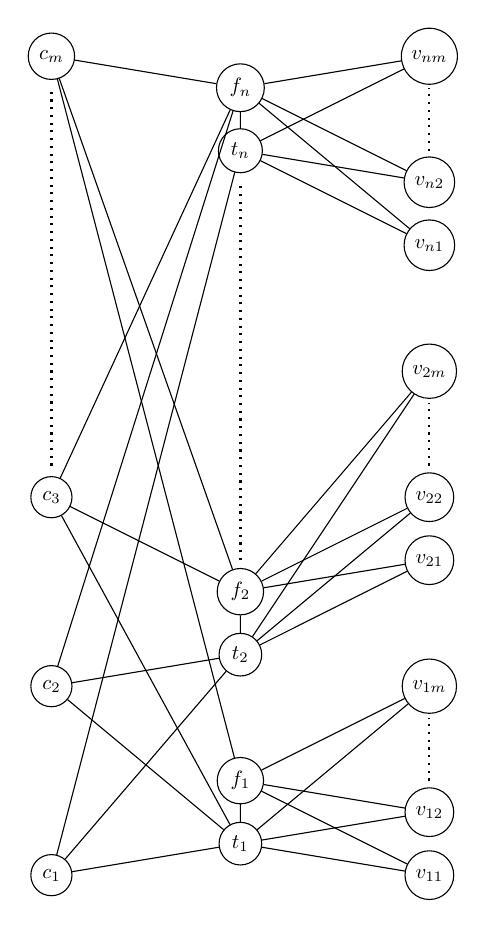
\begin{tikzpicture}
    [scale=0.8,auto=left,every node/.style={circle, draw, scale=0.75}]
    \node (c1) at (1,0) {$c_1$};
    \node (t1) at (4,0.5) {$t_1$};
    \node (f1) at (4,1.5) {$f_1$};
    \node (v11) at (7,0) {$v_{11}$};
    \node (v12) at (7,1) {$v_{12}$};
    \node (v1m) at (7,3) {$v_{1m}$};
    \node (c2) at (1,3) {$c_2$};
    \node (t2) at (4,3.5) {$t_2$};
    \node (f2) at (4,4.5) {$f_2$};
    \node (v21) at (7,5) {$v_{21}$};
    \node (v22) at (7,6) {$v_{22}$};
    \node (v2m) at (7,8) {$v_{2m}$};

    \node (c3) at (1,6) {$c_3$};
    \node (cm) at (1,13) {$c_m$};

    \node (tn) at (4,11.5) {$t_n$};
    \node (fn) at (4,12.5) {$f_n$};
    \node (vn1) at (7,10) {$v_{n1}$};
    \node (vn2) at (7,11) {$v_{n2}$};
    \node (vnm) at (7,13) {$v_{nm}$};

    \draw[dotted,thick] (1,6.5) -- (1,12.5);
    \draw[dotted,thick] (4,5) -- (4,11);
    \draw[dotted,thick] (7,1.5) -- (7,2.5);
    \draw[dotted,thick] (7,6.5) -- (7,7.5);
    \draw[dotted,thick] (7,11.5) -- (7,12.5);

    \foreach \from/\to in {c1/t1, c1/t2, c1/tn, c2/t1, c2/t2, c2/fn, c3/t1, c3/f2, c3/fn, cm/f1, 
      cm/f2, cm/fn,t1/f1, t2/f2,tn/fn, 
      v11/t1, v11/f1, v12/t1, v12/f1, v1m/t1, v1m/f1,
      v21/t2, v21/f2, v22/t2, v22/f2, v2m/t2, v2m/f2,
    vn1/tn, vn1/fn, vn2/tn, vn2/fn, vnm/tn, vnm/fn}
    \draw (\from) -- (\to);
  \end{tikzpicture}
  \caption{The transformation from 3SAT to SLRL}
  \label{transfo}
\end{figure}

Now we prove, that 3SAT has a solution if and only if SLRL has a solution. 
To prove the statement, it will be first shown, that if 3SAT has a solution SLRL also has a solution.
\begin{enumerate}
  \item{Assume 3SAT has a solution, that means we have a truth assignment, 
    which satisfies all the clauses.}
  \item{Construct the set of servers S as follows: If variable $u_j \in U$ is true
      in the truth assignment, then add $t_j$ to the server set. If variable $u_j \in U$
      is false, then add $f_j$ to the server set. Do this for each variable $u_j$ for $j = (1,\dots,n)$.
      As there are exactly n variables in U, this clearly satisfies our constraint 
    for k, i.e., the number of servers.}
  \item{At most m clauses inherit the variable $u_j$ and there are m vertices connected to every
      $t_j$ and $f_j$, i.e., $v_{ij}$ for $i=(1,\dots,m)$.
      Thus the number of vertices in the neighbor set is $m+m+2 = 2m+2 \leq r $ for every 
      $t_j$ or $f_j$. The additional two vertices result of the server and the respective 
    vertex representing the other truth value.}
  \item{The usage of each edge is at most one, which means it is smaller and equal to c. $1\leq c$.
    Thus it is obvious that this constraint is not violated.}
  \item{Consequently this instance of SLRL, (G,k,r,c) has a solution, because all constraints are satisfied 
    and as a result the first part of the equivalence is proven.}
\end{enumerate}
To finish our proof, we need to show the converse, i.e., 
if (G,k,r,c) is a solution there is also a solution for 3SAT. 

\begin{enumerate}
  \item{Assume (G,k,r,c) has a solution. Let $G_i, (i=1,\dots,n)$ be the subgraph induced
    by $t_i, f_i$ and $v_{ij},(j=1,\dots,m)$.}
  \item{We will now show, that there is only one way to place the servers, namely the truth
    value assignment for the variables, that satisfy the 3SAT instance}
  \item{Assume that there is no server in $G_i$. This would imply that the servers is a subset of
      $c_j$ for $(j=1\dots m)$. The problem there is, that not only is m $\neq$ n(concerning constraint k),
      but also that constraint c would be unsatisfied, because more than one path would use 
      the edge connecting $c_j$ and either $f_i$ or $t_i$ (there are m + 2 vertices in $G_i$).
    Thus placing a server on any $c_j$ is not possible, because it would automatically violate constraint c.}
  \item{Assume that the servers are placed on $v_{ij}$. This would also satisfy the neighborhood 
      constraint r, but it would certainly violate the constraint c, because the degree of $v_{ij}$ is two and
      and the number of vertices in $G_i$ is m+2. All of them would need to use one of the two edges for their shortest path,
    resulting in a violation.}
  \item{The only spare option that would satisfy the neighborhood constraint 
      are the vertices $t_i$ and $f_i$. Let $u_i$ be true if a server is located on
      $t_i$ and let $u_i$ be false if a server is located on $f_i$.  
      If an arbitrary $c_j$ has no adjacent vertice which is a server,
      the SLRL would not be fulfilled because there would be two shortest paths passing edge
      $(t_i,f_i)$. This would contradict $c = 1$ and also means that there is always an adjacent vertice which is a server to $c_j$.
      Therefore, the truth assignments satisfies all clauses.}
\end{enumerate}
Thus 3SAT was successfully reduced to SLRL in polynomial time.
Consequently, SLRL is NP-complete.$\square$

\section{SLRL as Optimization Problem}

After thoroughly discussing the decision problem of SLRL, the optimization problem
of SLRL will be tackled next. Like \cite{mirrorserver}, I decided to optimize the maximum 
neighborhood constraint considering the maximum usage of edges c.

\subsection{An Instance Of The Problem}
\begin{figure}[H]
  \centering
  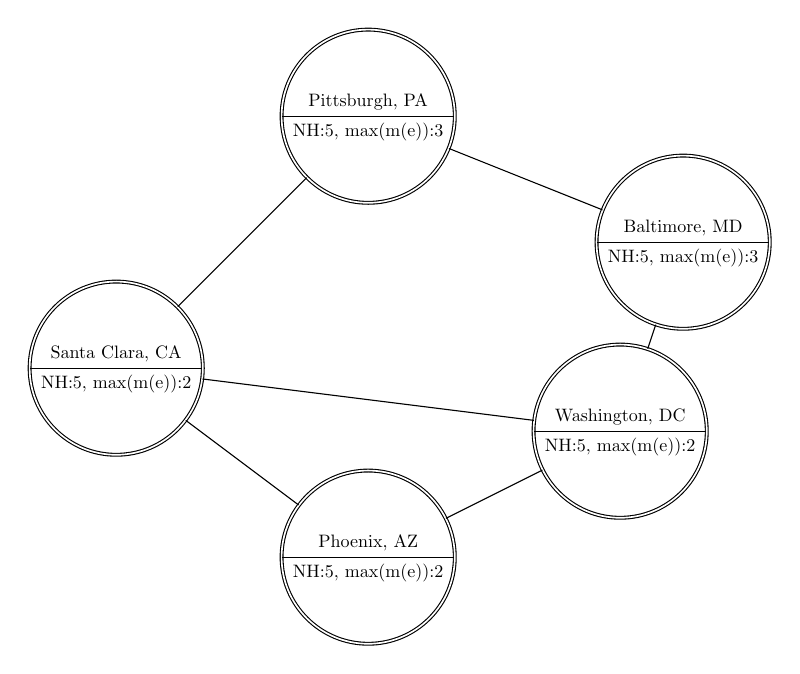
\begin{tikzpicture}
    [scale=0.8,auto=left,every node/.style={circle split, draw,double, scale=0.65}]
    \node (a) at (0,3) {Santa Clara, CA \nodepart{lower} NH:5, max(m(e)):2};
    \node (b) at (4,0) {Phoenix, AZ \nodepart{lower} NH:5, max(m(e)):2};
    \node (c) at (8,2) {Washington, DC \nodepart{lower} NH:5, max(m(e)):2};
    \node (d) at (9,5) {Baltimore, MD \nodepart{lower} NH:5, max(m(e)):3};
    \node (e) at (4,7) {Pittsburgh, PA \nodepart{lower} NH:5, max(m(e)):3};
    \foreach \from/\to in {a/b, a/c, a/e, b/c, c/d, d/e}
    \draw (\from) -- (\to);
  \end{tikzpicture}
  \caption{GetNet International as an Instance of SLRL}
\end{figure}
The above shown graph is from the barebone network "GetNet International".
It is parsed out of a dataset of barebone networks provided by caida \cite{caidabarebones}.
\\
The nodes have two values in their lower part: "NH and max(m(e))". NH stands for 
the maximum neighbourhood if that node was chosen as a server. Choosing the first
server obviously implicates the maximum neighbourhood, because there are
no mirror servers yet on the graph.\\
The multiplicity of an edge e, $m(e)$ is explained above. The number after
$max(m(e))$ in the lower part of the node describes $max(m(e)$ $ \forall e \in E)$,
if one decides to take this node as a server.
The greedy algorithm takes the node with the lowest $max(m(e))$ first.

\section{Implementation}


\subsection{Greedy Algorithms}
The only prior algorithm for this problem is the greedy algorithm proposed by
Miwa et al. \cite{mirrorserver}. It greedily puts the vertex with the 
lowest maximal neighbourhood if the constraint $c\geq m(e) (\forall e \in E)$ is fulfilled into the server set. 
Otherwise it will choose a vertex as server where $max_{e \in E}m(e)$ is the minimum.
\begin{algorithm}[H]
  \caption{GreedyLocation}
  \begin{algorithmic}[2]
    \Require G = (V,E), k, c 
    \State $S \gets \emptyset$
    \While {$|S| < k$}
    \State Choose vertex $v$ such that the
    maximum size of the neighbor sets of
    $S \cup \{v\}$ is the minimum
    for all vertices $v \in V$
    under the constraint that $m(e) \leq c$
    for all edges $e$. If there is no vertex 
    satisfying this constraint, choose v
    under the constraint that $max_{e \in E}m(e)$
    is the minimum.
    \State $S \gets S \cup \{ v \}$
    \EndWhile
    \If{$max_{e \in E}m(e) > c}$
    \State output infeasible
    \EndIf\\
    \Return S
  \end{algorithmic}
\end{algorithm}
The runtime of the original algorithm is $\mathcal O(kn^{2}*(V+E))$,
where $m = |E|$ and $n = |V|$. Seen  in general it is $\mathcal O(k * updateConstraints)$. 
In the paper \cite{mirrorserver}, the constraints calculation works like this:
To determine the shortest paths from one node to every other node takes 
$\mathcal O(V+E)$ using Breadth-First Search. This needs to be done for every node once,
which implies a runtime of $\mathcal O(n*(V+E))$. 
This calculations suffice to determine the size of the maximum neighbor set r . To determine the maximum
edge usage, every node (except the nodes in the server set) needs to be looked 
at again (the usage of the edges in the
path(s) to the server(s) need to be incremented, and a path can maximally be the whole graph), 
which results in a runtime of $\mathcal O(n^{2}*(V+E))$.   
This process is executed for every server added, thus resulting in the final runtime of
$\mathcal O(kn^{2}*(V+E))$. 
\subsection{A faster greedy algorithm: GreedyDegree}
Having seen greedy location yet another greedy algorithm is proposed namely GreedyDegree. This algorithm always chooses the vertex with the
highest degree first and puts it in the server set(obviously only if it is not already in the server set). This does not pose
a terrible solution because choosing nodes with a high degree often imply a lower usage of edges because it is well connected. It is obviously not very complicated 
and thus produces worse results than GreedyLocation but its runtime is much better ($\mathcal O(V*E)$). It is also observed how 
the two algorithms perform in combination with the tabu search and the simulated annealing algorithm in the last section. 
\begin{algorithm}[H]
  \caption{GreedyDegree}
  \label{greedydeg}
  \begin{algorithmic}[2]
    \Require G = (V,E), k, c 
    \State $S \gets \emptyset$
    \While {$|S| < k$}
    \State Choose vertex $v$ such that the degree of the vertex is maximal
    and $v \notin S$.
    \EndWhile
    \If{$max_{e \in E}m(e) > c}$
    \State output infeasible
    \EndIf\\
    \Return S
  \end{algorithmic}
\end{algorithm}

\subsection{Determination of the neighbour sets of a server and loads of the links}
As briefly described in the last section, when a server is added to the server set, the size of the maximum neighbor set r and
$ max_{e \in E}m(e)$ (namely the maximum usage of all edges) need to be recalculated, as the shortest paths from the nodes 
to the servers change. I tried to speed up the constraint calculation, 
because on a big graph it took a lot of time and also for local search algorithms the constraints need to be calculated
far more often than k times (servers need to be swapped a lot, implying a need for a faster constraint calculation).
My approach was to calculate all the paths before adding servers and also to save the edges used in the paths.
This is indeed in $\mathcal O(n^{3}*(V+E))$, but constraint calculation after adding and removing a server is much faster,
because the edges used are already saved and every node knows it's nearest server(s) in $\mathcal O(|S|)$. Saving 
every edge used in every path shortest path to the respective servers enabled me to do the constraint calculation without using the breadth first search.
Which results in a runtime of $\mathcal O(kn*(V+E))$ which is a obviously faster than $\mathcal O(kn^{2}*(V+E))$ with the disadvantage of more memory usage.
$\mathcal O(V+E)$ results of the need to track the usages. Storing all the paths allows finding the nearest servers in $\mathcal O(|S|)$ but the load on the links 
still need to be calculated.

\subsection{Modified BFS}
The breadth first search needed to be modified enabling it to find all the shortest paths 
from one node to another, as we need to consider every shortest path in order to simulate
the worst case scenario regarding load on links. Also, to reconstruct the paths, a list of parent nodes is saved
in every node, when reached. The important step to get all the shortest paths to a node is saving the distance needed to reach it:
Doing this enables vertices who are expanded later, to also be parent of a vertice which already has a parent, where this parent was
expanded before the current vertice. This condition is expressed in the second if statement.
The runtime of BFS $\mathcal O(|V| + |E|)$, remains unmodified. In order to augment
the chance of correctness I wrote test cases that would check the algorithm.
These tests are to be found in the "Test" package.

\begin{algorithm}[H]
  \caption{BFS}
  \label{BFS}
  \begin{algorithmic}[2]
    \Require Graph(V,E) G, Node start
    \State clearParents();    // clear parents from previous BFS
    \State resetDistance();   // clear distances from previous BFS
    \State Queue$<$Node$>$ nodeQueue $\gets \emptyset;$
    \State Set$<$Node$>$ visited $\gets \emptyset;$
    \State visited.add(start);
    \State nodeQueue.push(start); // add the beginning node to the queue 
    \While {$\neg$nodeQueue.empty}
    \State Node curNode = nodeQueue.pop(); // Get first node of queue (FIFO)
    \State visited.add(curNode); // mark node as visited
    \For{Edge e : curNode.edges} //iterate through all edges  
    \If{$\neg$visited.contains(e.node2))}
    \State nodeQueue.push(e.node2);
    \State e.node2.distance(curNode.distance+1);
    \EndIf
    \If{e.node2.distance == curNode.distance+1}
    \State e.node2.addParent(curNode); // every shortest path is saved 
    \EndIf
    \EndFor
    \EndWhile
  \end{algorithmic}
\end{algorithm}

\subsection{Tabu Search}
The tabu search introduced by Glover in 1986 \cite{Glover:1986:FPI:15310.15311} is the first meta search heuristics I tried to use on SLRL.
The algorithm takes five parameters: The graph $G$, the solution
to start from $startingS$, the maximum size of the tabulist $t_{size}$, the iterations $iter$, the lower bound for the maximum neighborhood
$r*$ and the constraint for the maximum edge usage $c$.\\
The algorithm starts with adding $startingS$ to the tabulist.  
After setting $startingS$ as current and best Solution the following operations will be carried out $iter$ times: 
\begin{enumerate}
  \item{A neighbor solution $neighborS$ determined by algorithm \ref{localS} is obtained.}
  \item{The solution $neighborS$ is added to the tabulist.}
  \item{If the size of the tabulist is greater than $t_{size}$ the oldest element will be removed.}
  \item{The current solution $curS$ is set to be the $neighborS$ and it is then evaluated if it is the best Solution.}
  \item{If $curS$ is a better solution than $bestS$, i.e., if the maximum neighborhood of servers in $curS$, $r$, is lower than the respective counterpart in 
      $best$ and the maximum usage of edges is below $c$, $bestS$ is set to be $curS$. If the best solution is not solved, i.e., it does not fuilfill the
      maximum edge usage constraint $c$, only the maximum edge usage values,
    $bestS.lastC$ and $curS.lastC$ will be compared. If $curS.lastC$ is lower than $bestS.lastC$, it is the new best solution}
  \item{If the new solution satisfies the maximum edge usage constraint c and the maximum neighborhood is equal to $r*$, an optimal
    solution is found and the algorithm stops and returns the solution.}
\end{enumerate}
After completing the above described procedure $iter$ times $bestS$ is returned.
The implementation is shown in algorithm \ref{tabusa}. The datastructure used to represent the solution saves the maximum edge usage, the maximum neighborhood
of the solution and the solution itself, i.e., the set of servers. 

\begin {algorithm} [H]
\caption {tabu search}
\label {tabusa}
\begin {algorithmic} [3]
\Require Graph(V,E) G, Solution startingS, Tabulistsize $t_{size}$, Iterations iter, MaxEdgeUsage c, MaxNeighborhoodLowerBound r*
\State Solution curS;
\State Solution neighborS;
\State Solution bestS;
\State Tabulist l $\gets$ $\emptyset$
\State bestS = curS = startingS;
\State tabulist $\gets$ curS;
\For{i=0; i$<$iter; i++}
\State  neighborS = localSearch(curS, G, c, l); // described in Algorithm \ref{localS}
\State  tabulist $\gets$ neighborS;
\If {tabulist.size $>$ $t_{size}$}
\State removeOldestEntry();
\EndIf
\State  curS = neighborS;
\If{(curS.lastC $\leq$ c) $\&\&$ (curS.r $<$ bestS.r) }
\State bestSolution.setSolved(true);
\State bestSolution = currentSol;
\If{curS.getR()==r*}
\State break; // best possible feasible Solution found
\EndIf
\EndIf  
\If{($\neg$bestS.solved) $\&\&$ (bestS.lastC$>$curS.lastC) }
\State curS.setSolved(curS.lastC$\leq$c);
\State bestS = curS;
\EndIf 
\EndFor\\
\Return bestS;
\end {algorithmic}
\end {algorithm}
\subsection{The local search for the tabu search}
The local search algorithm displayed in algorithm \ref{localS} takes
the following three parameters as input (i) the solution to start from $curS$
(ii) the Graph $g$ to operate on and (iii) the limit for the maximum edge usage c.
The purpose of the algorithm is to create a neighborhood N by swapping servers in the solution
resulting in a different potentially better solution. If the new Solution is a new best Solution it is remembered as $bestS$.
The only difference to an ordinary local search algorithm is, that it minds the tabu list mentioned in algorithm \ref{tabusa}.
This means, that it will exchange the former best solution only if the new solution is not contained in the tabulist.
It starts with setting the server set of the graph to the server set in the starting solution. After that the whole
neighborhood induced by changing one server of the starting solution is looked at and the best solution is picked. As the first solution
is already in the tabulist, the best solution is not set in the beginning.
The following procedure is executed to create the neighborhood:
\begin{enumerate}
  \item{Start an outer loop and iterate over every server in the initial server set.}
  \item{Remove the server from the server set that is currently iterated over}
  \item{Iterate over every other node in the graph which is not a server and add it to the server set.}
  \item{Recalculate the constraints and if the solution is better than the last solution, exchange it.}
  \item{Remove the newly added node and continue with the next iteration of step 3.}
  \item{After step 3 iterated over every relevant node, add the removed server again and continue with the next iteration of step 1.}
\end{enumerate}

\begin {algorithm} [H]
\caption {localsearch}
\label {localS}
\begin {algorithmic} [3]
\Require Solution curS, Graph(V,E) g, MaxEdgeUsage c 
\State Solution bestS $\gets \emptyset$;
\State g.Servers $\gets$ curS.Servers;
\For{Node server : g.servers}
\State    g.removeServer(server);
\For{Node otherNode: g.nodes}
\If{(othernode $\neq$ server) $\wedge$ (otherNode $\notin$ g.servers)}
\State g.addServer(otherNode);
\State g.updateConstraints();
\State max\_usage = g.maxUsage; //the maximum usage of the edges
\State max\_neighbourset = g.MaxNeighbourSet; //size of biggest neighbor set
\If{(max\_usage $\leq$ c) $\wedge$ ((max\_neighbourset)$<$bestSolution.r)
$\wedge$(g.servers $\notin$ tabulist) }
\State bestSolution=new Solution(g.servers,max\_neighbourset,max\_usage,true);
\EndIf 
\If{($\neg$bestSolution.solved) $\wedge$ (bestSolution.lastC$>$max\_usage)
$\wedge$ (g.servers $\notin$ tabulist)}
\State bestSolution=new Solution(g.servers,max\_neighbourset,max\_usage, max\_usage$\leq$c);
\EndIf
\State g.removeServer(otherNode);
\EndIf
\EndFor
\State g.addServer(server);
\EndFor\\
\Return  bestS;
\end {algorithmic}
\end {algorithm}

\subsection{Simulated Annealing}
Simulated Annealing described in algorithm \ref{simA} is another heuristic approach, introduced by Kirkpatrick et al. \cite{Kirkpatrick83optimizationby}, that
was applicated to tackle the SLRL-Problem. Simulated Annealing allows 
escaping the local optima by initially allowing worse solutions than the initial solution and then by lowering the temperature with some time (which steers the allowance probability for worse solutions)
only allowing the better solutions.
This feature is a result of using the metropolis criterion as stated in algorithm \ref{metcrit}.
As input parameters an initial solution $initS$, a graph $g$, the maximal usage of an edge $c$, the lowerbound for the maximum neighborhood $r*$,
the desired runtime $r_{sec}$, the temperature $t_{init}$ and the cooling factor c is required.
After assigning the initial temperature and $initS$ to the variable $temp$ and $initS$ to $solX$,
the algorithm executes a while loop for a minimum of $r_{sec}$ seconds:
\begin{enumerate}
  \item {A random neighbor solution is generated and saved to variable $solY$}
  \item {The new random solution $solY$ is compared to the old solution $solX$. A function $compareSolution(.,.)$ takes care of 
    comparing the values of the maximum neighbor set and the maximum edge usage.}
  \item {If the solution is better, the new solution is set to be solX.}
  \item {If it is not better, the solutions are compared with the metropolis criterion. The code for the criterion is stated in algorithm \ref{metcrit}. If the metropolis criterion
    is fulfilled the new solution is also set to be solX. }
  \item {The temperature is decremented, which results in a lower chance for the metropolis criterion.}
  \item {If the runtime of the loop is not more than $r_{sec}$ go to step one.}
\end{enumerate}
After the loop, $solX$ is returned.


\begin {algorithm} [H]
\caption {Simulated Annealing}
\label {simA}
\begin {algorithmic} [3]
\Require Solution initS, Graph(V,E) g, MaxEdgeUsage c, Runtime $r_{sec}$, Temperature $t_{init}$, Cooling factor c,
Lowerbound\_r $r*$; 
\State Temperature temp = $t_{init}$;
\State Solution solX = initS; 
\While{timepassed $<$ $r_{sec}$}
\State Solution solY = randomNeighbor(solX);
\If{compareSolutions(solX,solY)} // if solY is better than solX
\State solX = solY;
\Else
\If{metropoliscriterion(solX,solY,temperature)}
\State solX = solY; // see algorithm \ref{metcrit}
\EndIf
\EndIf    
\State temp = temp*c; // cooling takes place here
\If{(solX.r==$r*$) $\wedge$ (solX.lastC $\leq$ c)}
\State break;
\EndIf 
\EndWhile\\
\Return solX;
\end {algorithmic}
\end {algorithm}

The Metropolis Criterion described in algorithm \ref{metcrit} allows simulated annealing to escape local optima. When a new solution is not better 
than the current solution, it may still be replaced with the current solution under a certain probability,
namely $p_{accept}=e^{-|rating(y)-rating(x)|/T}$. $rating(.)$ is a function displayed at algorithm \ref{rating}, which rates the quality of a solution under the condition
that rating(x) $>$ 0, where x is a solution for the SLRL. T is the current temperature. If the new solution y is only slightly worse than solution x and the temperature T is very high,
the chance for replacement is higher than with a lower temperature.

\begin {algorithm} [H]
\caption {Metropolis Criterion}
\label {metcrit}
\begin {algorithmic} [3]
\Require Solution y, Solution x, Temperature T
\State Z = random Number $\in [0,1)$
  \If {$Z<e^{-|rating(y)-rating(x)|/T}$} \Comment see Algorithm \ref{rating}\\
  \Return true;
  \EndIf\\
  \Return false;
  \end {algorithmic}
  \end {algorithm}

  Rating a solution is done as described in algorithm \ref{rating}. It is highly valued, if the solution is
  feasible. The other part of the rating is done by adding the ratios of (i) the lower bound of maximum neighbor sets and the current maximum of neighbor sets and
  (ii) the ratio of the limit of the maximum edge usage and the current maximum edge usage.
  \begin {algorithm} [H]
  \caption {Rating}
  \label {rating}
  \begin {algorithmic} [3]
  \Require Solution x, MaxEdgeUsage c, LowerBound r\_lower
  \State rating = 0;
  \State //solution is valid
  \If {x.lastC$<$c}
  rating += 1;
  \EndIf
  \State rating+=c/x.lastC;
  \State rating+=r\_lower/x.r);\\
  \Return rating;

  \end {algorithmic}
  \end {algorithm}

  \section{Performance Evaluation}

  \subsection{Data (test instances)}
  The data taken for the performance evaluation is from caida \cite{caidabarebones}. Parsing the
  data was not as trivial as it sounds, because the data is not formatted well,
  and several modifications have been done to fit the problem.
  Unfortunately the syntax proposed in the beginning of the file is not considered
  for each and every network, because different people added networks to the file.
  I also modified the data to make it fit for the problem and to approximate the
  data of the paper \cite{mirrorserver} as best as I could:
  \begin{itemize}
    \item If the graph G given for the barebone network was not connected,
      the connected component with less nodes of that graph is cut out.
    \item Normally the connected cities are listed in the following manner:
      "city,state,country" and in order to match with the number of Nodes and Edges
      in the paper \cite{mirrorserver} only city and state are used for
      identification and the country is left out. Sometimes London
      is used on one hand as City in Canada and on the other hand in GB, denoted like this
      London, *, Canada and London, *, England. They are differentiated.
    \item Sometimes the State has a number. One example would be "Kansas City, KS2~"
      This is interpreted as "Kansas City, KS".
  \end{itemize}

  All those modifications were done to match the graphs of \cite{mirrorserver} as closely as possible.
  As I did not have the data of the other paper, I tried to match them with the number of
  nodes and number of vertices. Unfortunately three instances of my instances do not
  match the number of nodes and / or vertices proposed from the paper mentioned.
  The varying instances are: "Sprint", "Cable and Wireless" and "UUNet".

  \subsection{Evaluation}
  In the following section, the performance of the described algorithms is evaluated. The data used is described in the previous section.
  In \cite{mirrorserver} a way of defining the constraints given G=(V,E) is stated which was used for this evaluation as well: 
  \begin{itemize}
    \item{The number of servers $k = \lceil |V| * 0.1 \rceil$  }
    \item{The limit of the maximum usage for every edge $c = \lceil(\frac{|V|}{(k*\Delta)}*d)\rceil$. $\Delta$ is the maximum degree and $d$ is a positive integer.}
    \item{The lower bound of the maximum usage for every edge $c\_lower = \lceil(\frac{|V|}{(k*\Delta)})\rceil$. $\Delta$ is the maximum degree.}
    \item{The lower bound of the maximum size of the neighbor sets $r*=\frac{|V|}{k}$.}
  \end{itemize}
  In \cite{mirrorserver} $d$ is defined as four. %They defined a solution as solved if $\frac{r}{r*}$ was no more than two, and the maximum usage for every edge was below $c$.% 
  The following pages show performance evaluations of the algorithm.  Three instances could not be solved, because the maximum usage of the 
  edges was bigger than c. A simple algorithm which enumerates all the solutions for an instance and checks the constraints was written and was not able to find a feasible solution 
  for the instance "Allegiance Telecom". The instances  "AT\&T WorldNet" and "UUNet" are also instances which are unsolved. Unfortunately they are too big to be solved by enumeration so
  nothing can be said about them in this regard. In table \ref{table:compalgs} one can see the numerical results of the algorithms on the instances provided by caida. When no
  feasible solution was found for a specific instance the value is marked with -. n is the number of vertices, m the number of edges. The number displayed for each algorithm is r, i.e.,%abbreviations gl glts gdts %
  the size of the maximum neighbor set of each server which is also the value we want to optimize. As shown by table \ref{table:compalgs}, better results for 15 out of 38 instances could be obtained 
  by either the tabu search or the simulated annealing algorithm. With $d$ being four one instance is not solvable, namely Allegiance Telecom. 
  The two instances AT\&T WorldNet and UUNet remain unsolved. For UUNet an infeasible solution could be found with an maximum edge usage of three, when two is required. 
  For AT\&T WorldNet the best infeasible solution regarding maximum edge usage found is four, but two is required for a feasible solution. 
  Two more instances could be solved using the new algorithms (they are solved by every of the new algorithms), namely BBN Planet and PSINet.
  The barchart in figure \ref{bar3algs} displays the results graphically. If an algorithm has not solved a specific instance its bar will not be shown in the chart.
  The following abbreviations have been used to describe the algorithms that have been used to solve the instance. GL stands for Greedy Location, GL+TS means that first Greedy Location was used 
  to obtain a solution for the instance and then the tabu search was executed to optimize it. GD+SA similarly means that Greedy Degree was used to solve the instance and Simulated Annealing was in then used
  to search for a better solution. In figure \ref{gd-gl-ts} and figure \ref{gd-gl-sa} the greedy location and greedy degree algorithm are compared when used in combination with simulated
  annealing and tabu search. The instances shown are the respective tested instances where differences in performance can be seen. In all other tested instances the results are the same. 
  We can see that greedy degree performs a bit worse in three of the five cases and that it performs better in the other two cases where results differ.


  \newpage  
  \thispagestyle{empty}
  \begin{table}[H]
  \scalebox{0.9}{
    \begin{tabular}{ | l | l | l | l | l | l | l | l | l | l | }
      \hline
      Networks                    & n   & m   & k   & r*  & GL   & GL+TS    & GL+SA   & GD+TS   & GD+SA \\ \hline
      above.net                   & 22  & 25  & 3   & 8   &  13  &  13      &  13     & 13      & 13  \\ \hline
      At Home Network             & 46  & 55  & 5   & 10  &  11  &  10      &  10     & 11      & 10  \\ \hline
      AGIS                        & 82  & 92  & 9   & 10  &  14  &  11      &  11     & 11      & 11  \\ \hline
      AT\&T WorldNet              & 93  & 154 & 10  & 10  &  -   &   -      &   -     &  -      &  - \\ \hline
      BBN Planet                  & 41  & 49  & 5   & 9   &  -   &   13     &   13    &  13     &  13 \\ \hline
      Cable Internet              & 8   & 7   & 1   & 8   &  8   &   8      &   8     &  8      &  8  \\ \hline
      CAIS Internet               & 37  & 44  & 4   & 10  &  12  &   10     &   10    &  10     &  10 \\ \hline
      CompuServe Network Services & 16  & 23  & 2   & 8   &  11  &   10     &   10    &  10     &  10 \\ \hline
      CRL Network Services        & 35  & 50  & 4   & 9   &  12  &   12     &   12    &  12     &  12 \\ \hline
      DataXchange Network, Inc.   & 8   & 24  & 1   & 8   &  8   &   8      &   8     &  8      &  8  \\ \hline
      Allegiance Telecom          & 53  & 88  & 6   & 9   &  -   &   -      &    -    &   -     &  - \\ \hline
      EPOCH Networks, Inc.        & 29  & 30  & 3   & 10  &  14  &  14      &    14   &   14    &  14 \\ \hline
      EUnet                       & 28  & 30  & 3   & 10  &  23  &  23      &    23   &   23    &  23 \\ \hline
      Exodus                      & 14  & 19  & 2   & 7   &  9   &  9       &    9    &   9     &  9  \\ \hline
      Genuity                     & 48  & 53  & 5   & 10  &  14  &  12      &    11   &   12    &  11 \\ \hline
      GeoNet Communications, Inc. & 13  & 15  & 2   & 7   &  10  &  10      &    10   &   10    &  10 \\ \hline
      GetNet International        & 5   & 6   & 1   & 5   &  5   &  5       &    5    &   5     &  5  \\ \hline
      GlobalCenter                & 9   & 36  & 1   & 9   &  9   &  9       &    9    &   9     &  9  \\ \hline
      GoodNet                     & 27  & 58  & 3   & 9   &  20  &  19      &    19   &   19    &  19 \\ \hline
      IDT Corp                    & 15  & 18  & 2   & 8   &  9   &  9       &    8    &   9     &  8  \\ \hline
      ipf.net                     & 5   & 5   & 1   & 5   &  5   &  5       &    5    &   5     &  5  \\ \hline
      iSTAR Internet Inc.         & 20  & 22  & 2   & 10  &  14  &  14      &    14   &   14    &  14 \\ \hline
      Cable \& Wireless           & 20  & 34  & 2   & 10  &  12  &  12      &    10   &   11    &  10 \\ \hline
      MindSpring                  & 41  & 45  & 5   & 9   &  22  &  22      &    22   &   22    &  22 \\ \hline
      Nap.Net, LLC                & 6   & 7   & 1   & 6   &  6   &  6       &    6    &   6     &  6  \\ \hline
      Netrail Incorporated        & 17  & 21  & 2   & 9   &  12  &  11      &    11   &   11    &  11 \\ \hline
      PSINet                      & 78  & 110 & 8   & 10  &   -  &  18      &    16   &   14    &  16 \\ \hline
      Qwest                       & 14  & 26  & 2   & 7   &   8  &  8       &    8    &   8     &  9  \\ \hline
      RISQ Network                & 13  & 12  & 2   & 7   &   8  &  8       &    8    &   8     &  8  \\ \hline
      RNP                         & 27  & 35  & 3   & 9   &   12 &  12      &    12   &   12    &  12 \\ \hline
      Savvis Communications       & 28  & 56  & 3   & 10  &   20 &  19      &    19   &   19    &  19 \\ \hline
      ServInt Internet Services   & 23  & 34  & 3   & 8   &   12 &  11      &    11   &   11    &  11 \\ \hline
      Sprint                      & 21  & 37  & 3   & 7   &   11 &  9       &    9    &   9     &  9  \\ \hline
      Telstra Internet            & 21  & 24  & 3   & 7   &   13 &  13      &    13   &   13    &  13 \\ \hline
      UUNET                       & 126 & 316 & 13  & 10  &  -   &  -       &     -   &    -    &  - \\ \hline
      Verio                       & 35  & 72  & 4   & 9   &  17  &   17     &    17   &    17   &  17 \\ \hline
      VisiNet                     & 11  & 13  & 2   & 6   &  10  &   7      &    7    &    7    &  7  \\ \hline
      XO Communications           & 33  & 38  & 4   & 9   &  16  &   11     &    11   &    12   &  12 \\ \hline
    \end{tabular}
    }
    \caption{Comparison of the Algorithms}
    \label{table:compalgs}
  \end{table}
  \thispagestyle{empty}

\begin{figure}[H]
  \begin{center}
    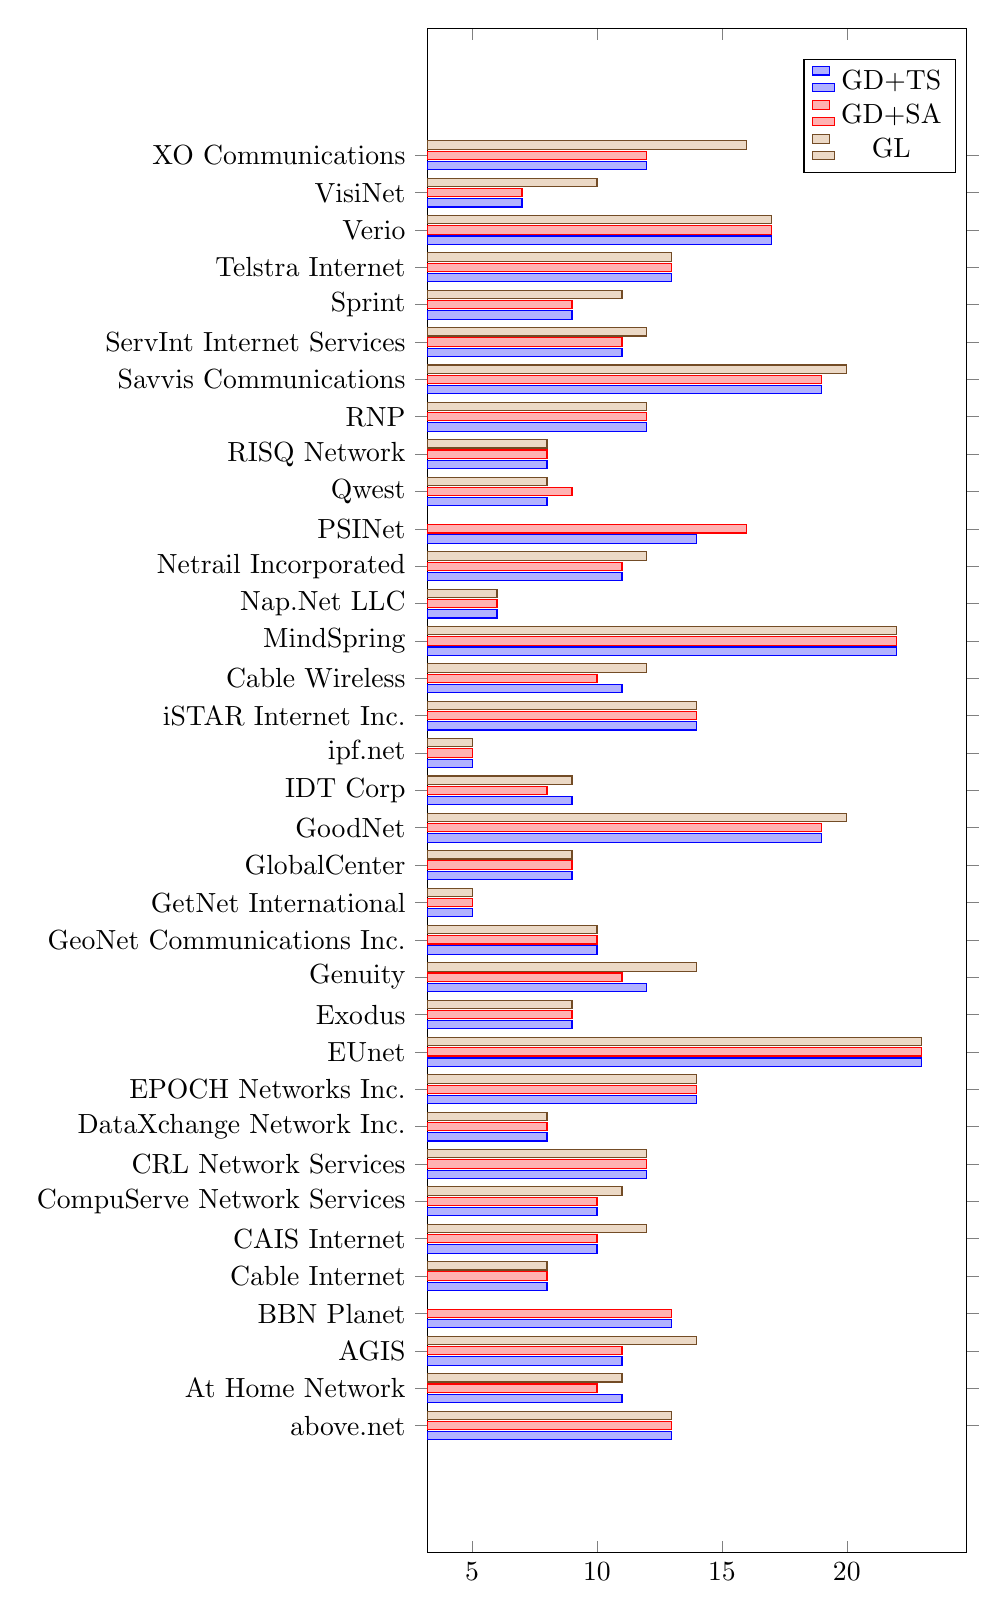
\begin{tikzpicture}
      \begin{axis}[
          symbolic y coords={
            above.net,
            At Home Network,
            AGIS,
            BBN Planet,
            Cable Internet,
            CAIS Internet,
            CompuServe Network Services,
            CRL Network Services,
            DataXchange Network Inc.,
            EPOCH Networks Inc.,
            EUnet,
            Exodus,
            Genuity,
            GeoNet Communications Inc.,
            GetNet International,
            GlobalCenter,
            GoodNet,
            IDT Corp,
            ipf.net,
            iSTAR Internet Inc.,
            Cable  Wireless,
            MindSpring,
            Nap.Net LLC,
            Netrail Incorporated,
            PSINet,
            Qwest,
            RISQ Network,
            RNP,
            Savvis Communications,
            ServInt Internet Services,
            Sprint,
            Telstra Internet,
            Verio,
            VisiNet,
            XO Communications,
          },
          y=13.5,
          ytick=data,
          y tick label style={/pgf/number format/1000 sep=},
          xbar=0.7pt,
          %xbar=0.7pt,
          bar width=3pt
        ]
        %TS + GD
        \addplot coordinates {
          (13,above.net)
          (11,At Home Network)
          (11,AGIS)
          (13,BBN Planet)
          (8,Cable Internet)
          (10,CAIS Internet)
          (10,CompuServe Network Services)
          (12,CRL Network Services)
          (8,DataXchange Network Inc.)
          (14,EPOCH Networks Inc.)
          (23,EUnet)
          (9,Exodus)
          (12,Genuity)
          (10,GeoNet Communications Inc.)
          (5,GetNet International)
          (9,GlobalCenter)
          (19,GoodNet)
          (9,IDT Corp)
          (5,ipf.net)
          (14,iSTAR Internet Inc.)
          (11,Cable  Wireless)
          (22,MindSpring)
          (6,Nap.Net LLC)
          (11,Netrail Incorporated)
          (14,PSINet)
          (8,Qwest)
          (8,RISQ Network)
          (12,RNP)
          (19,Savvis Communications)
          (11,ServInt Internet Services)
          (9,Sprint)
          (13,Telstra Internet)
          (17,Verio)
          (7,VisiNet)
          (12,XO Communications)
        };

        %%GD + SA
        \addplot coordinates {

          (13,above.net)
          (10,At Home Network)
          (11,AGIS)
          (13,BBN Planet)
          (8,Cable Internet)
          (10,CAIS Internet)
          (10,CompuServe Network Services)
          (12,CRL Network Services)
          (8,DataXchange Network Inc.)
          (14,EPOCH Networks Inc.)
          (23,EUnet)
          (9,Exodus)
          (11,Genuity)
          (10,GeoNet Communications Inc.)
          (5,GetNet International)
          (9,GlobalCenter)
          (19,GoodNet)
          (8,IDT Corp)
          (5,ipf.net)
          (14,iSTAR Internet Inc.)
          (10,Cable  Wireless)
          (22,MindSpring)
          (6,Nap.Net LLC)
          (11,Netrail Incorporated)
          (16,PSINet)
          (9,Qwest)
          (8,RISQ Network)
          (12,RNP)
          (19,Savvis Communications)
          (11,ServInt Internet Services)
          (9,Sprint)
          (13,Telstra Internet)
          (17,Verio)
          (7,VisiNet)
          (12,XO Communications)        
        };
        %%greedy location
        \addplot coordinates {
          (13,above.net)
          (11,At Home Network)
          (14,AGIS)
          (8,Cable Internet)
          (12,CAIS Internet)
          (11,CompuServe Network Services)
          (12,CRL Network Services)
          (8,DataXchange Network Inc.)
          (14,EPOCH Networks Inc.)
          (23,EUnet)
          (9,Exodus)
          (14,Genuity)
          (10,GeoNet Communications Inc.)
          (5,GetNet International)
          (9,GlobalCenter)
          (20,GoodNet)
          (9,IDT Corp)
          (5,ipf.net)
          (14,iSTAR Internet Inc.)
          (12,Cable  Wireless)
          (22,MindSpring)
          (6,Nap.Net LLC)
          (12,Netrail Incorporated)
          (8,Qwest)
          (8,RISQ Network)
          (12,RNP)
          (20,Savvis Communications)
          (12,ServInt Internet Services)
          (11,Sprint)
          (13,Telstra Internet)
          (17,Verio)
          (10,VisiNet)
          (16,XO Communications)
        };
        \legend{GD+TS,GD+SA,GL}
      \end{axis}
    \end{tikzpicture}
  \end{center}
  \caption{Comparison of Greedy Location(GL),Greedy Degree with Tabu Search(GD+TS), Greedy Degree with Simulated Annealing(GD+SA)}
  \label{bar3algs}
\end{figure}
\thispagestyle{empty}


\begin{figure}[H]
  \begin{center}
    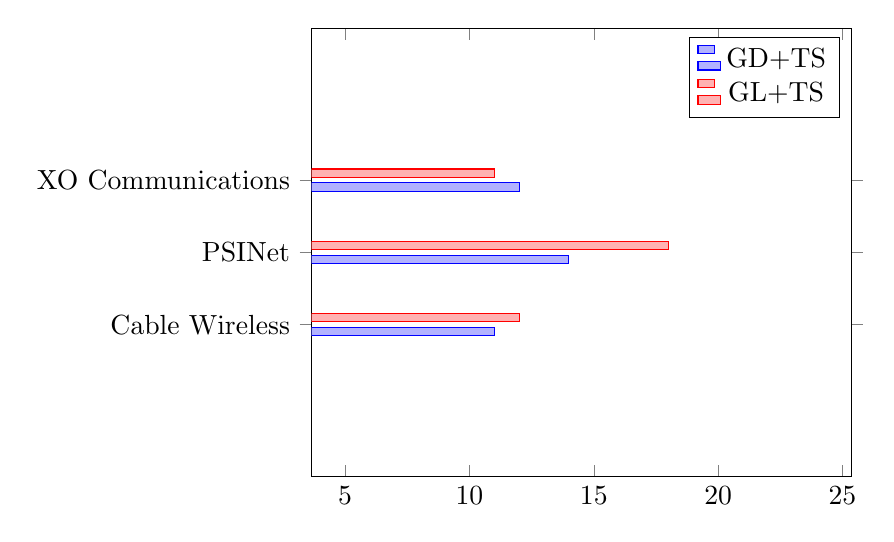
\begin{tikzpicture}
      \begin{axis}[
          symbolic y coords={
            Cable  Wireless,
            PSINet,
            XO Communications,
          },
          ytick=data,
          y tick label style={/pgf/number format/1000 sep=},
          xbar,
          enlargelimits=1.05,
          bar width=3pt
        ]
        %gd
        \addplot coordinates{
          (11,Cable  Wireless)
          (14,PSINet)
          (12,XO Communications)
        };
        %gl
        \addplot coordinates{
          (12,Cable  Wireless)
          (18,PSINet)
          (11,XO Communications)
        };
        \legend{GD+TS, GL+TS}
      \end{axis}
    \end{tikzpicture}
  \end{center}
  \caption{Comparison of Greedy Location with Tabu Search(GL+TS) and Greedy Degree with Tabu Search(GD+TS)}
  \label{gd-gl-ts}
\end{figure}
\thispagestyle{empty}


\begin{figure}[H]
  \begin{center}
    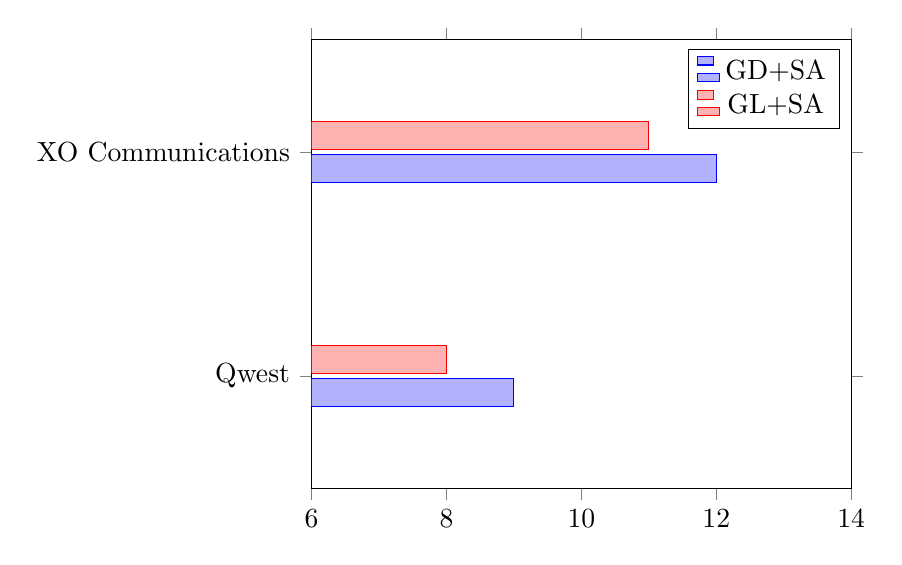
\begin{tikzpicture}
      \begin{axis}[
          symbolic y coords={
            Qwest,
            XO Communications,
          },
          ytick=data,
          y tick label style={/pgf/number format/1000 sep=},
          ybar,
          enlargelimits=0.5,
          xbar
          %xbar=0.7pt,
        ]
        %GD
        \addplot coordinates{
          (9,Qwest)
          (12,XO Communications)
        };
        %GD
        \addplot coordinates{
          (8,Qwest)
          (11,XO Communications)
        };
        \legend{GD+SA,GL+SA}
      \end{axis}
    \end{tikzpicture}
  \end{center}
  \caption{Comparison of Greedy Location with Simulated Annealing(GL+SA) and Greedy Degree with Simulated Annealing(GD+SA)}
  \label{gd-gl-sa}
\end{figure}
\thispagestyle{empty}

\bibliography{bibtex}

\end{document}
